\onehalfspacing

\section{Struttura}


Il firewall controller può potenzialmente essere posizionato in un qualsiasi punto della rete. Le regole sono specificate nella tabella di flusso che sono gestite sia dallo switch che dal firewall controller (vedi tabella \ref{fig:flow}). Una voce nella tabella di flusso corrisponde ad una regola che gestisce il flusso del traffico. Lo switch agisce come un banale inoltratore di pacchetti basato sulle regole di sicurezza definite nella sua tabella di flusso. Il firewall controller utilizza la sua tabella di flusso per tenere traccia delle decisioni intraprese sul traffico.

Un canale di comunicazione dedicato viene mantenuto tra lo switch e il controller del firewall. Attraverso questo canale, lo switch invia le informazioni sui flussi di traffico non identificati al controller per l'ispezione e il controller invia le decisioni allo switch.

\begin{figure}[H]
  \centering
    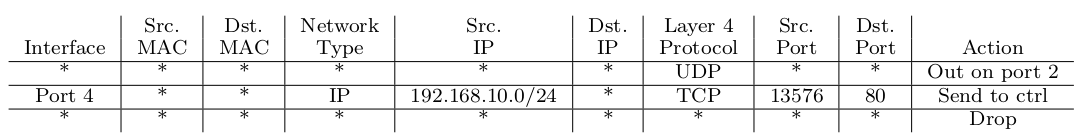
\includegraphics[width=\linewidth]{img/flow.png}
    \caption{Esempio di Tabella di Flusso (Flow Table)}
  \label{fig:flow}
\end{figure}

\section{Modalità Permissiva e Restrittiva}

Sono state presenti due modalità per specificare le azioni di controllo predefinite in base al traffico:

\begin{itemize}
  \item \textbf{\textit{Modalità permissiva:}} rifiuto selettivo dei flussi. Ossia che il traffico viene normalmente inoltrato di default a meno che non venga esplicitamente negato.
  \item \textbf{\textit{Modalità restrittiva:}} autorizzazione selettiva dei flussi. Ossia che il traffico viene negato di default a meno che esplicitamente consentito.
\end{itemize}


\section{First Deny Last Allow}
Un controller firewall adotta una metodologia \textit{"first deny last allow"} per determinare un'azione di controllo su un flusso.

Un controller privilegia flusso che "matcha" (corrisponde) ad una regola di rifiuto (deny rule) rispetto a una regola di permissiva (allow rule). La precedenza delle regole di rifiuto sulle regole di consenso allevia il rischio per la sicurezza derivante da regole potenzialmente in conflitto nella tabella di flusso del controller ed anche evita che i pacchetti debbano percorrere un'intero set di regole prima di essere scartati.


\section{Posizione delle regole: Valutazione delle performances}

In seguito verranno brevemente presentate le prestazioni di un firewall di rete basato su regole. In genere, e come mostrato nella Figura \ref{fig:firewallrulebase}1, i pacchetti in entrata che trasportano richieste arrivano al firewall e vengono messi in coda per l'elaborazione in più fasi:

\begin{enumerate}
  \item La prima fase prevede l'esecuzione di funzionalità di collegamento dati e livello di rete.
  \item Successivamente viene attivato il motore di ricerca delle regole del firewall per elaborare i pacchetti in entrata.
\end{enumerate}

Salah cita da un'altra fonte \cite{salah2011performance} che è stato dimostrato che le regole in fondo alla tabella possono essere scoperte da un aggressore esterno. Un utente malintenzionato può quindi lanciare un attacco che prenda di mira principalmente le regole di in fondo alla tabella e degradi efficacemente e rapidamente le prestazioni di un firewall con una serie di attacchi DoS a basso volume di traffico. Questo tipo di attacco viene chiamato "attacco di complessità algoritmica" (Complexity-algorithmic attacks), è una classe di attacchi DoS a bassa velocità che sfruttano le carenze algoritmiche nella progettazione del software \cite{salah2011performance}.

Risulta quindi importante capire che impatto possono avere questi attacchi sulle prestazioni dei firewall in modo da trovare modi per mitigare il problema.

\subsection{Misure prese}

Il tema di Salah ha effettuato le misurazioni sottoponendo il firewall a due tipi di traffico: traffico normale e traffico DDoS indirizzato a regole diverse situate in posizioni diverse nell'insieme di regole del firewall.
\newline
\newline
In base all'hardware a disposizione del team è stato misurato che:
\begin{itemize}
  \item Il valore medio era di circa 0,5 ms per l'interrogazione di 10.000 regole, ossia 0,05 microsecondi per singola regola.
  \item Il tempo medio di elaborazione del kernel del driver del dispositivo e dell'elaborazione IP ed è stato riscontrato che il valore medio è di circa 2,65 microsecondi.
\end{itemize}

\begin{figure}[H]
  \centering
    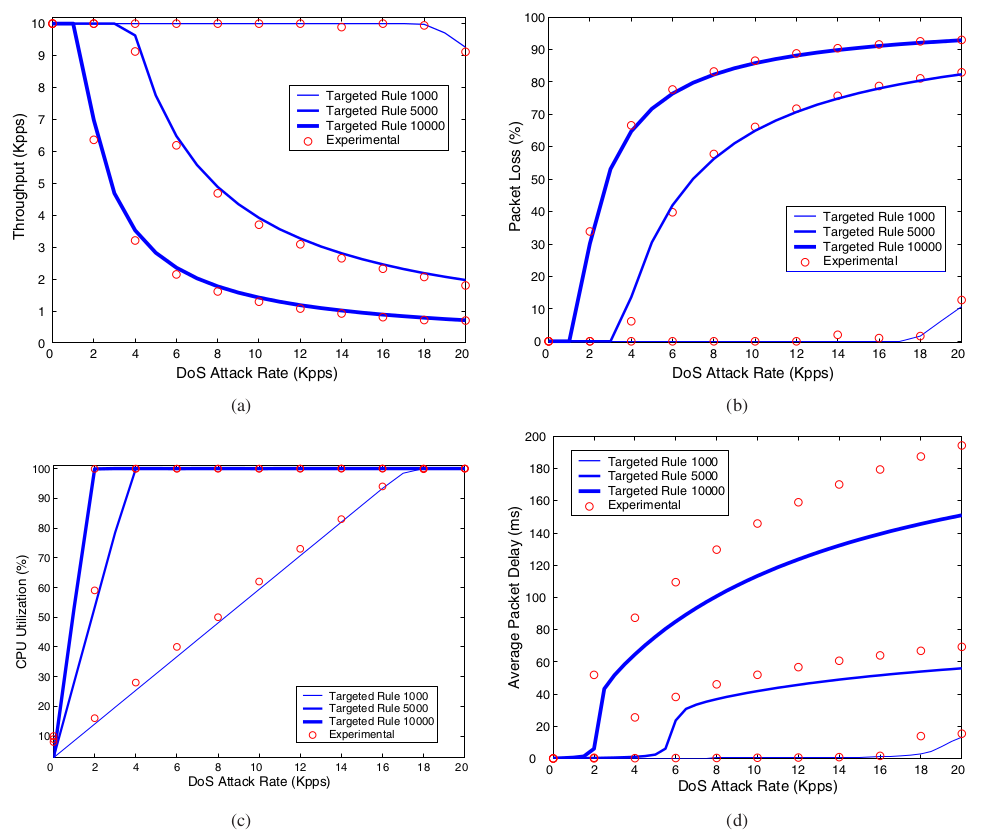
\includegraphics[width=\linewidth]{img/dos.png}
    \caption{L'impatto dei flussi di traffico DoS che colpiscono diverse regole sul firewall}
  \label{fig:dos}
\end{figure}

La Figura \ref{fig:dos} mostra l'impatto sulle prestazioni che il firewall subisce quando si lanciano attacchi DoS con velocità diverse che colpiscono posizioni diverse delle regole. L'impatto è stato misurato facendo in modo che venga generato un normale flusso di traffico UDP costante a una velocità di 10 Kpps.

Abbiamo misurato il degrado delle prestazioni in termini di perdita di pacchetti (packet loss), velocità effettiva, utilizzo della CPU e ritardo unidirezionale quando si invia traffico normale e quando si sottopone il firewall a flussi di attacchi DoS di velocità diverse e prendendo di mira regole diverse.

\subsection{Osservazioni}

Dai grafici mostrati in Figura \ref{fig:dos} emerge chiaramente che un leggero degrado si manifesta quando gli attacchi DoS prendono di mira le regole più importanti (quelle in cima), mentre un notevole degrado si manifesta quando gli attacchi DoS colpiscono regole meno importanti (quelle in fondo) come quelle posizionate a 5.000 e 10.000. Più specificamente, quando si prendono di mira le regole meno importanti, si può osservare un degrado grave e evidente con attacchi DoS a velocità relativamente bassa di circa 1 Kpp e 3 Kpp quando si prendono di mira regole posizionate rispettivamente a 10.000 e 5.000. Tuttavia, quando si prende di mira una regola posizionata a 1000, il degrado si manifesta solo con attacchi DoS ad alta velocità di circa 18 Kpps.

Pertanto, si può concludere che le regole di targeting nella parte inferiore del set di regole possono essere gravemente dannose per le prestazioni del firewall. Le prestazioni del firewall sono accettabili quando gli attacchi DoS (fino a una velocità di 18 Kpps) mirano a regole posizionate intorno a 1.000, ma non a regole superiori.

\section{Conotroller: Valutazione delle performances}

Nella valutazione, il team di Collins fa uso di una configurazione restrittiva con insiemi di regole composte completamente da regole permissive (allow rules). Ciò rappresenta il caso di regole base peggiore perché il controller del firewall è costretto a tentare di accettare ogni flusso di traffico non identificato.

Il numero di regole nelle configurazioni varia da un minimo di 3 a un massimo di 1000.

\begin{figure}[H]
  \centering
  \begin{subfigure}[b]{0.46\linewidth}
    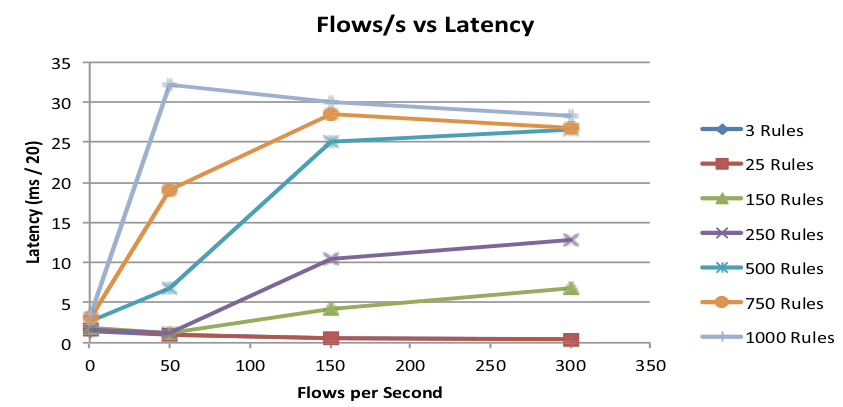
\includegraphics[width=\linewidth]{img/flow_latency.png}
    \caption{Crescita della latenza media}
    \label{fig:flowlatency}
  \end{subfigure}
  \begin{subfigure}[b]{0.46\linewidth}
    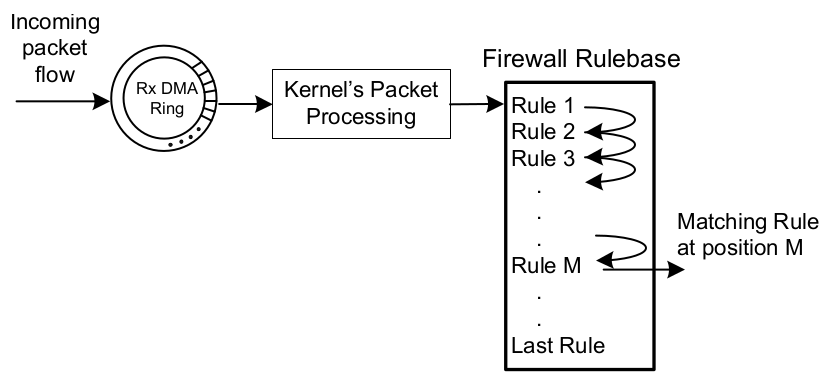
\includegraphics[width=\linewidth]{img/firewall_rulebase.png}
    \caption{Schema di interrogazione delle regole del firewall per i pacchetti in arrivo}
    \label{fig:firewallrulebase}
  \end{subfigure}
\end{figure}

Dal grafico \ref{fig:flowlatency} si osserva che la latenza media aumenta linearmente con il tasso di arrivo di nuovi flussi di traffico quando la dimensione del set di regole è 150. Le latenze medie mostrano improvvisi aumenti di latenza con un numero più alto di arrivi di flussi quando le dimensioni del set di regole è a 250 e 500. La latenza media smette di crescere quando il set di regole è a 750 e 1000.

Questa interruzione di crescita, secondo Collins può essere dovuta principalmente a due motivi:

\begin{enumerate}
  \item Molti nuovi flussi di traffico hanno pattern molto simili, quindi dopo un iniziale processamento da parte del controller le regole per quel pattern vengono applicate allo switch. Questa cosa viene osservata spesso in molti flussi di traffico di un gateway principale dove per esempio, molte connessioni Web tentano di visitare lo stesso insieme di server (per esempio portali di News molto frequentati).
  \item Molti flussi vengono scartati (dropped) a causa dello spazio di coda limitato per contenere i pacchetti dei flussi non identificati quando i tassi di arrivo dei flussi sono elevati. La latenza media mostrata in tabella non copre i flussi persi.
\end{enumerate}

